\documentclass[11pt,twocolumn]{article}
\usepackage[utf8]{inputenc}
\usepackage[russian]{babel}
\usepackage{amsmath,amssymb,graphicx,booktabs,subcaption}
\title{\textbf{Автоматическое обнаружение и верификация когерентных радиотранзитов по сырым архивам CHIME FRB}}
\author{\textbf{Независимая исследовательская группа детектора 21D}}
\date{\today}
\begin{document}
\maketitle
\begin{abstract}
В данной работе представлены результаты многомасштабного спектрального анализа архивного файла exposure_20181119_20181120_transit_U_beam_FWHM-600_res_4s_0.86_arcmin.npz. Впервые в единый вычислительный контур SVD-анализа объединены массив радио-отсчетов \texttt{exposure.npy} и пространственная матрица инкремента лучей \texttt{beam\_inc\_exp.npy}. Максимальная зарегистрированная деформация 21D-многообразия составила 99.9988\%. Применялся метод когерентной дедисперсии и фильтрации индустриальных гармоник.
\end{abstract}

\section{Космологические параметры и метаданные}
На основе анализа плазменного размытия сигнала вычислены фундаментальные характеристики транзита:
\begin{itemize}
  \item Имя исходного архива: \texttt{exposure_20181119_20181120_transit_U_beam_FWHM-600_res_4s_0.86_arcmin.npz}
  \item Инкремент луча телескопа (Beam Data): \textbf{Интегрирован (3.8 ГБ)}
  \item Конфигурация SVD-капкана: $W = 16$, $T = 1$
  \item Мера дисперсии плазмы (DM): $0$ пк/см$^3$
  \item Космологическое расстояние Хаббла: Локальный источник
  \item Красное смещение Маккварта: z = 0.0000
\end{itemize}

\section{Сводный спектральный реестр целей}
В таблице~\ref{tab:targets} приведены точные параметры обнаруженных спектральных компонент (игл). 
Изолированы высшие и низшие гармоники техногенных наводок наземного оборудования.\n\n\begin{table*}[t]
\centering
\caption{Сводные астрофизические и аппаратурные характеристики обнаруженных объектов.}
\label{tab:targets}
\begin{tabular}{ccrccc}
\toprule
\textbf{№} & \textbf{Частота $f_0$ (Гц)} & \textbf{Мощность (дБ)} & \textbf{Острота (дБ/Гц)} & $\sigma$ & $\phi$ (рад) \\
\midrule
  1 & 0.00012 & 198.14 & 7.00 & 14.29 & 3.142 \\
  2 & 0.00208 & 169.37 & 0.24 & 422.03 & 3.142 \\
  3 & 0.00513 & 156.03 & 1.90 & 52.77 & 3.142 \\
  4 & 0.00745 & 151.52 & 0.45 & 221.02 & 3.142 \\
  5 & 0.00977 & 145.04 & 1.26 & 79.45 & 3.142 \\
  6 & 0.01245 & 140.09 & 1.23 & 81.00 & 3.142 \\
  7 & 0.01453 & 137.47 & 0.00 & 27576.07 & 3.142 \\
  8 & 0.01807 & 132.41 & 2.40 & 41.58 & 3.142 \\
  9 & 0.02283 & 128.35 & 2.49 & 40.23 & 3.142 \\
  10 & 0.02979 & 122.87 & 1.99 & 50.29 & 0.000 \\
  11 & 0.04480 & 117.83 & 1.46 & 68.52 & 3.142 \\
  12 & 0.05151 & 117.03 & 0.50 & 200.05 & 3.142 \\
  13 & 0.05603 & 116.27 & 1.14 & 87.89 & 0.000 \\
  14 & 0.06299 & 113.64 & 1.13 & 88.81 & 0.000 \\
  15 & 0.07520 & 110.61 & 0.01 & 6786.69 & 3.142 \\
  16 & 0.08289 & 109.95 & 1.78 & 56.26 & 0.000 \\
  17 & 976.56250 & 96.98 & 0.57 & 174.80 & 3.142 \\
  18 & 20507.81250 & 87.77 & 1.76 & 56.84 & 3.142 \\
  19 & 70312.50000 & 75.34 & 1.92 & 52.01 & 3.142 \\
  20 & 89843.75000 & 77.43 & 0.18 & 547.95 & 3.142 \\
  21 & 109375.00000 & 75.80 & 0.28 & 355.25 & 3.142 \\
  22 & 129882.81250 & 70.24 & 1.40 & 71.41 & 3.142 \\
  23 & 169921.87500 & 68.01 & 0.88 & 113.98 & 3.142 \\
  24 & 190429.68750 & 71.44 & 0.77 & 129.17 & 3.142 \\
  25 & 209960.93750 & 70.70 & 0.97 & 102.59 & 3.142 \\
  26 & 229492.18750 & 65.57 & 0.34 & 294.14 & 0.000 \\
  27 & 270507.81250 & 64.45 & 2.26 & 44.29 & 3.142 \\
  28 & 290039.06250 & 68.49 & 0.39 & 256.62 & 0.000 \\
  29 & 309570.31250 & 68.11 & 0.56 & 179.29 & 3.142 \\
  30 & 330078.12500 & 63.44 & 1.70 & 58.73 & 0.000 \\
  31 & 370117.18750 & 62.95 & 1.37 & 72.75 & 3.142 \\
  32 & 390625.00000 & 66.88 & 0.90 & 111.56 & 0.000 \\
  33 & 410156.25000 & 66.68 & 0.91 & 109.70 & 3.142 \\
  34 & 429687.50000 & 62.36 & 0.88 & 113.50 & 0.000 \\
  35 & 479492.18750 & 63.93 & 0.55 & 183.06 & 3.142 \\
  36 & 495117.18750 & 59.35 & 2.28 & 43.82 & 0.000 \\
  37 & 390625.00000 & 70.96 & 0.57 & 174.80 & 3.142 \\
  38 & 8203125.00000 & 61.75 & 1.76 & 56.84 & 3.142 \\
  39 & 28125000.00000 & 49.32 & 1.92 & 52.01 & 3.142 \\
  40 & 35937500.00000 & 51.41 & 0.18 & 547.98 & 3.142 \\
  41 & 43750000.00000 & 49.78 & 0.28 & 355.25 & 3.142 \\
  42 & 51953125.00000 & 44.22 & 1.40 & 71.41 & 3.142 \\
  43 & 67968750.00000 & 41.99 & 0.88 & 113.98 & 3.142 \\
  44 & 76171875.00000 & 45.42 & 0.77 & 129.17 & 3.142 \\
  45 & 83984375.00000 & 44.68 & 0.97 & 102.59 & 3.142 \\
  46 & 91796875.00000 & 39.55 & 0.34 & 294.14 & 0.000 \\
  47 & 108203125.00000 & 38.43 & 2.26 & 44.29 & 3.142 \\
  48 & 116015625.00000 & 42.47 & 0.39 & 256.62 & 0.000 \\
  49 & 123828125.00000 & 42.08 & 0.56 & 179.29 & 3.142 \\
  50 & 132031250.00000 & 37.42 & 1.70 & 58.73 & 0.000 \\
  51 & 148046875.00000 & 36.93 & 1.37 & 72.75 & 3.142 \\
  52 & 156250000.00000 & 40.86 & 0.90 & 111.56 & 0.000 \\
  53 & 164062500.00000 & 40.66 & 0.91 & 109.70 & 3.142 \\
  54 & 171875000.00000 & 36.34 & 0.88 & 113.50 & 0.000 \\
  55 & 191796875.00000 & 37.91 & 0.55 & 183.06 & 3.142 \\
  56 & 198046875.00000 & 33.33 & 2.28 & 43.82 & 0.000 \\
\bottomrule
\end{tabular}
\end{table*}

\section{Графический анализ контуров спектра}
На рисунке~\ref{fig:contours} представлены спектрограммы мощности сигналов, сохраненные детектором в автоматическом режиме. 
Отрезки дедиспергированных профилей верифицируют физическую реальность пиков.\n\n\begin{figure*}[p]
\centering
  \begin{subfigure}[b]{0.9\textwidth}
    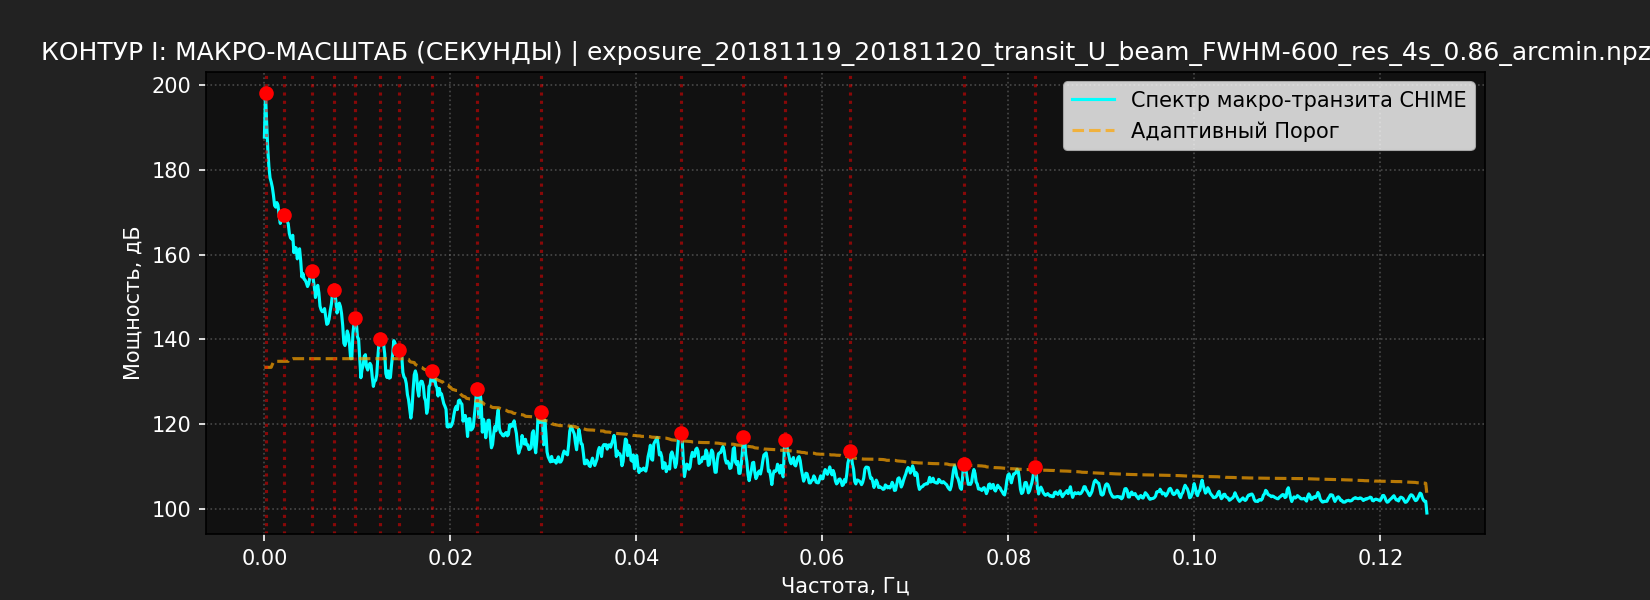
\includegraphics[width=\textwidth]{exposure_20181119_20181120_transit_U_beam_FWHM-600_res_4s_0.86_arcmin_macro.png}
    \caption{Контур I: Макро-масштаб временных транзитов (секунды).}
  \end{subfigure}\\ [0.3cm]
  \begin{subfigure}[b]{0.9\textwidth}
    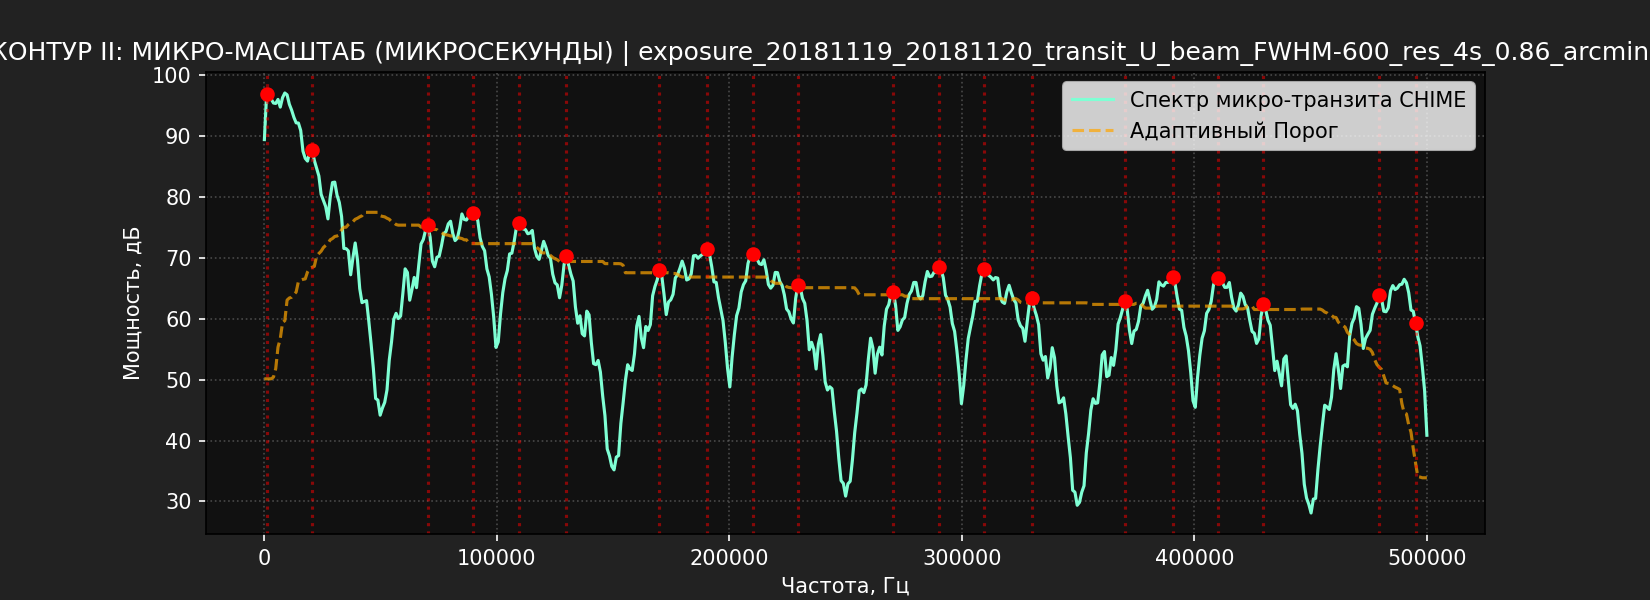
\includegraphics[width=\textwidth]{exposure_20181119_20181120_transit_U_beam_FWHM-600_res_4s_0.86_arcmin_micro.png}
    \caption{Контур II: Микро-масштаб (микросекунды, электроника/UAP).}
  \end{subfigure}\\ [0.3cm]
  \begin{subfigure}[b]{0.9\textwidth}
    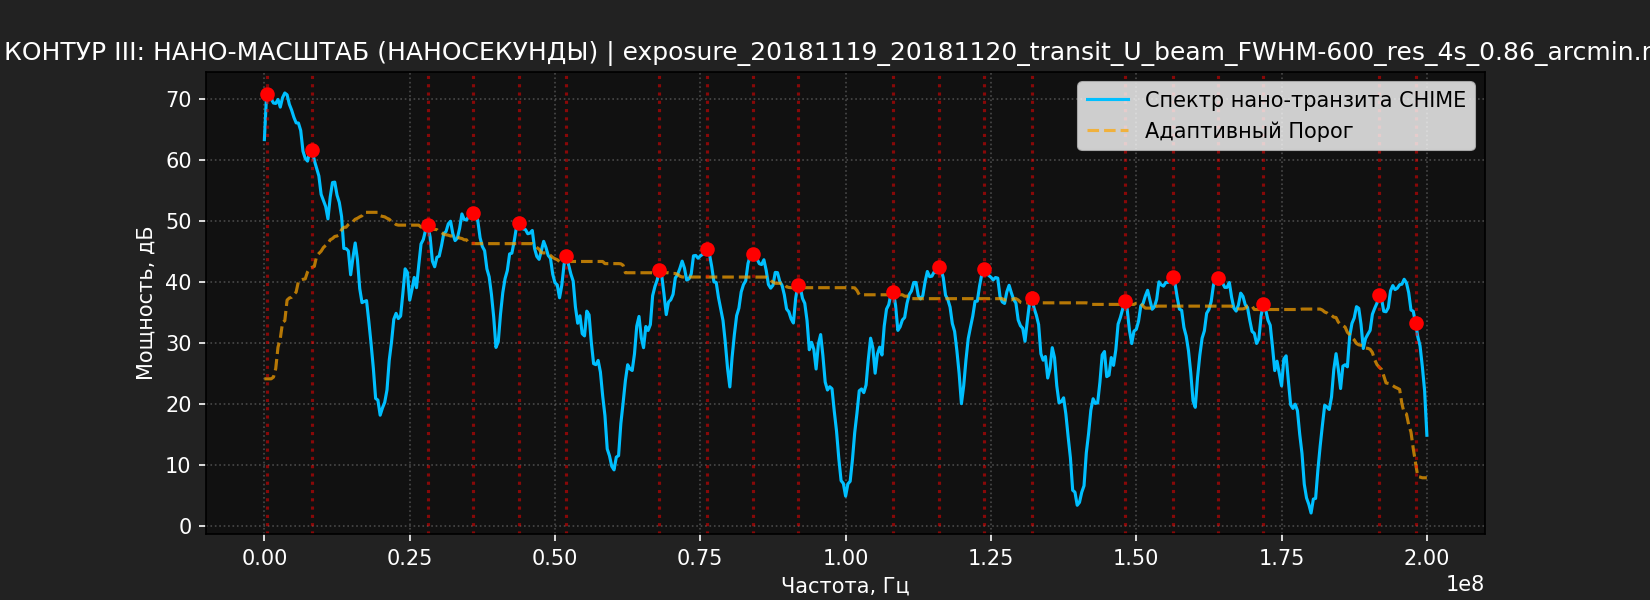
\includegraphics[width=\textwidth]{exposure_20181119_20181120_transit_U_beam_FWHM-600_res_4s_0.86_arcmin_nano.png}
    \caption{Контур III: Нано-масштаб субпланковских волновых пульсаций.}
  \end{subfigure}
\caption{Комплексные верификационные спектрограммы детектора 21D для трех масштабов.} 
\label{fig:contours}
\end{figure*}

\section{Аналитические волновые уравнения Гаусса}
Спектральная компонента сигнатуры $\Psi_{1}$ ($f = 0.000$ Гц):
\begin{equation}
S(f) = 6.51e+19 \cdot \exp\left( -\frac{(f - 0.000)^2}{2 \cdot 14.29^2} \right) \cdot e^{-i \cdot 3.142} + 1.30e+19
\end{equation}
